% Two harnesses compose into one harness. The composite contains the two harnesses whole
% (each keeps its contract, parameters, evidence and monitors) and adds its own layer.
% Same shapes as single-harness.tex.   Build: pdflatex harness-composition.tex
\documentclass[border=8pt]{standalone}
\usepackage[T1]{fontenc}
\usepackage[default]{sourcesanspro}
\usepackage{amsmath,amssymb}
\usepackage{sansmath}
\usepackage{tikz}
\usetikzlibrary{arrows.meta}
\definecolor{wrap}{HTML}{92C7E7}
\definecolor{outer}{HTML}{C9E3F3}
\definecolor{edge}{HTML}{2F5B7C}
\definecolor{navy}{HTML}{14273A}
% wrapper: fill, x, y, width, height, snip
\newcommand{\wrapper}[6]{\draw[fill=#1,draw=edge,line width=1.5pt]
  (#2,#3)--++(#4,0)--++(0,{#5-#6})--++(-#6,#6)--++({-#4+2*#6},0)--++(-#6,-#6)--cycle;}
% code block: x, y, width, height
\newcommand{\codeblock}[4]{\draw[fill=white,draw=navy,line width=1.2pt]
  (#1,{#2+#4})--++(#3,0)--++(0,{-0.83*#4})
  .. controls ++({-0.32*#3},0) and ++({0.22*#3},0) .. ++({-0.72*#3},{-0.17*#4})
  .. controls ++({-0.11*#3},0) and ++({0.09*#3},{-0.03*#4}) .. ++({-0.28*#3},{0.06*#4})--cycle;}
% one whole harness: x, y, index
\newcommand{\harness}[3]{%
  \wrapper{wrap}{#1}{#2}{4.6}{4.8}{0.75}
  \node[font=\bfseries\large,text=navy] at ({#1+2.3},{#2+4.35}) {Harness #3};
  \node[chip] at ({#1+1.25},{#2+3.6}) {contract $C_{#3}$};
  \node[chip] at ({#1+3.35},{#2+3.6}) {parameters $P_{#3}$};
  \node[chip] at ({#1+1.25},{#2+2.95}) {evidence $E_{#3}$};
  \node[chip] at ({#1+3.35},{#2+2.95}) {monitors};
  \codeblock{#1+0.7}{#2+0.55}{3.2}{1.95}
  \node[font=\bfseries\large,text=navy] at ({#1+2.3},{#2+1.7}) {C++ code #3};}
\begin{document}
\sansmath
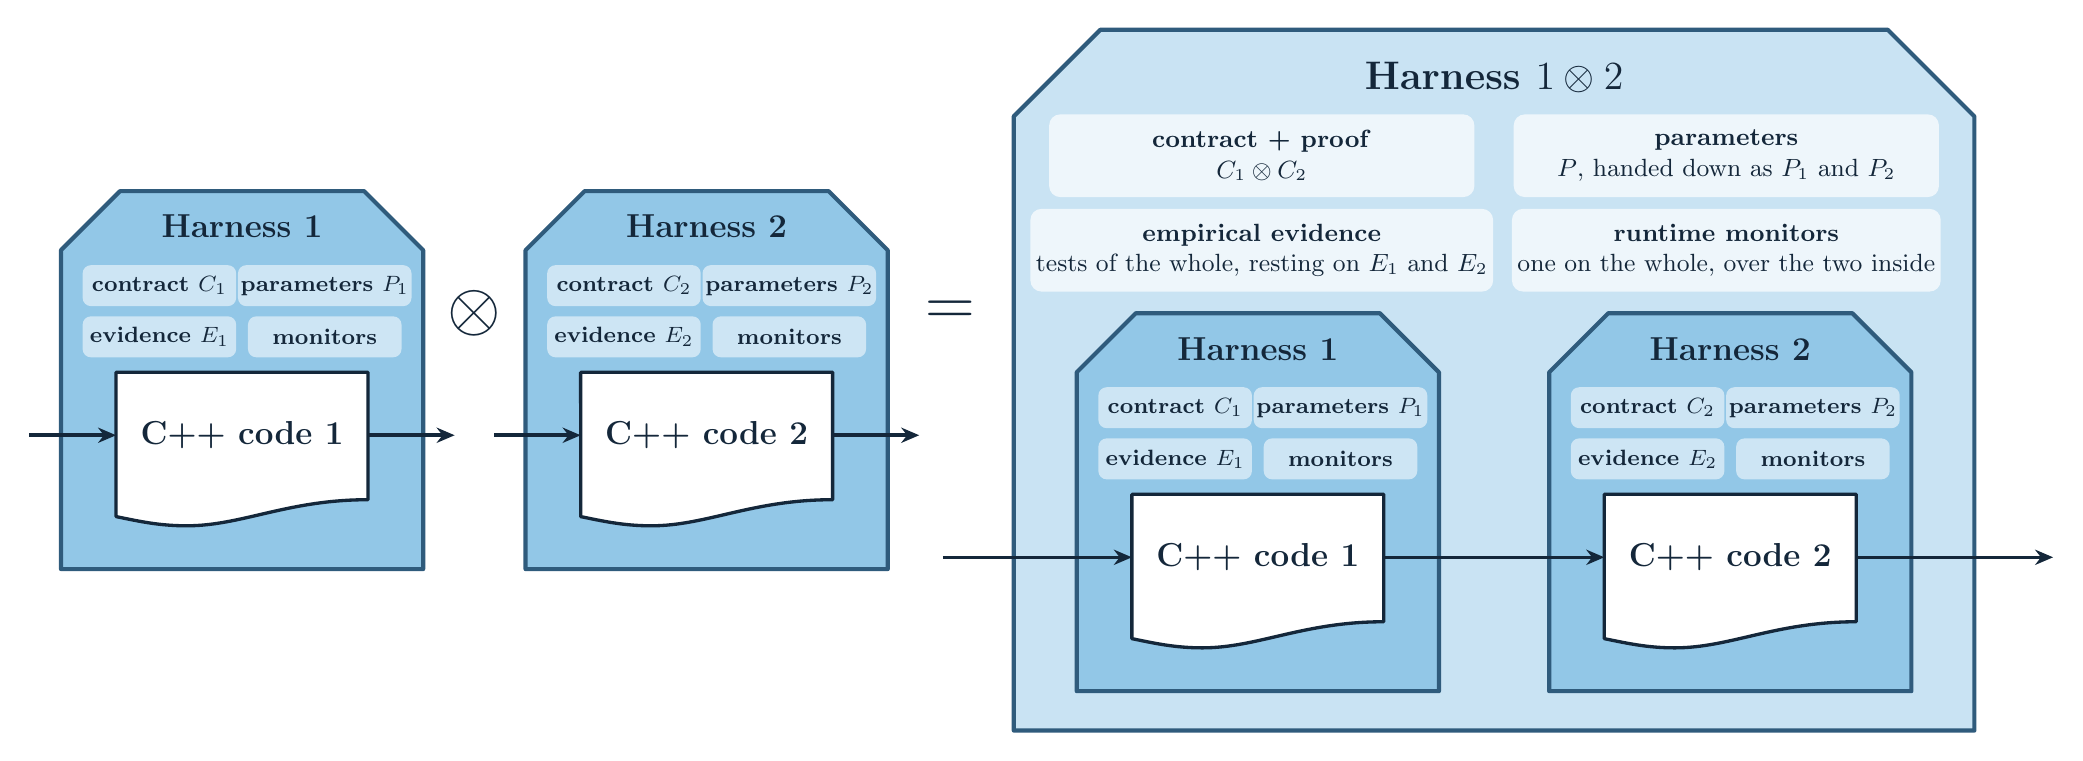
\begin{tikzpicture}[x=1cm,y=1cm,>={Stealth[length=6.5pt,width=5.5pt]},line join=round,
  chip/.style={fill=white,fill opacity=0.55,text opacity=1,rounded corners=3pt,text=navy,
               minimum width=1.95cm,minimum height=0.52cm,font=\bfseries\footnotesize,inner sep=1pt},
  item/.style={fill=white,fill opacity=0.7,text opacity=1,rounded corners=4pt,text=navy,
               minimum width=5.4cm,minimum height=1.05cm,align=center,font=\small,inner sep=2pt},
  wire/.style={line width=1.3pt,navy}]

% ---------- the two harnesses
\harness{0}{2.05}{1}
\harness{5.9}{2.05}{2}
\foreach \x in {0,5.9}{
  \draw[wire,->] (\x-0.4,3.75)--(\x+0.7,3.75);
  \draw[wire,->] (\x+3.9,3.75)--(\x+5.0,3.75);}
\node[font=\Huge,text=navy] at (5.25,5.3) {$\otimes$};
\node[font=\Huge,text=navy] at (11.3,5.3) {$=$};

% ---------- the composite: a harness around the two harnesses
\wrapper{outer}{12.1}{0}{12.2}{8.9}{1.1}
\node[font=\bfseries\Large,text=navy] at (18.2,8.3) {Harness $1\otimes 2$};
\node[item] at (15.25,7.3) {\textbf{contract + proof}\\$C_1\otimes C_2$};
\node[item] at (21.15,7.3) {\textbf{parameters}\\$P$, handed down as $P_1$ and $P_2$};
\node[item] at (15.25,6.1) {\textbf{empirical evidence}\\tests of the whole, resting on $E_1$ and $E_2$};
\node[item] at (21.15,6.1) {\textbf{runtime monitors}\\one on the whole, over the two inside};
\harness{12.9}{0.5}{1}
\harness{18.9}{0.5}{2}
\draw[wire,->] (11.2,2.2)--(13.6,2.2);
\draw[wire,->] (16.8,2.2)--(19.6,2.2);
\draw[wire,->] (22.8,2.2)--(25.3,2.2);
\end{tikzpicture}
\end{document}
